\chapter{Foundation}
\label{chap:foundation}


%-outlines three different ship operations
%-discusses possibilities of on-board training on each
%-one is chosen for prototyping and evaluation based on some criteria
%-
%

This chapter covers results of a domain analysis that was conducted to derive requirements for a scenario-based ship crew training method. The contents of this chapter are relevant to answering the research question - what are operational scenarios in which mixed reality training could be useful. A prototype was envisaged to evaluate the feasibility of the training method described here. Prototypes inevitably embody a particular design choice; a choice rife with challenges faced by systems design described below in section \ref{sec:designchallenge}. This study deals with the challenge by first outlining a few design choices. Consequently, one is chosen for prototyping and evaluation. 
%Results can then be viewed in light of the general context.

A manoeuvre training scenario was chosen for prototyping and evaluation despite the high level of photorealism thought to be required for the concept to be workable. The reasoning for this choice two-fold. Firstly, an evaluation (user-testing a prototype) in this scenario would bring to light shortcomings, if any, of state-of-the-art consumer grade AR devices for their ability to render high quality 3D graphics necessary to create believable augmented reality training scenarios. Secondly, manoeuvring scenarios in offshore supply context do not require a large number of virtual objects in the scene. Position keeping for example, is an exercise where the vessel is to be kept stationary with reference to a particular offshore construction. Position keeping training scenario then allowed for rapid prototyping with low time-investment on developing the virtual aspect of the augmented reality.

Section \ref{sec:operationaldemands} titled operational demands describe from an operator point-of-view, requirements for safe execution of ship handling operations. In designing a technological solution, the SCE method takes into account human factors that could affect interactions between users and the system being developed. Section \ref{sec:humanfactors} titled human factors knowledge describes mode errors - a type of error arising from the operation of state-dependent systems out of state. Finally, section \ref{sec:envisionedtech} describes technological options available to implement the augmented reality training method that is envisioned and  their pros and cons.
%A literature survey on the topic of augmented reality in maritime context brings up studies of applications that aid job performance by providing helpful contextual information on top of real-world views. Overlaying route way-points, distance to next way-point, local hazards and other navigational aids allows the integration of various information that is used by the officer of the watch into one single augmented display. In poor visibility conditions, virtual rails on both sides of the ship help with steering. Buoys, fog signals, day beacons and other navigational aids can also be visually overlaid in low-visibility conditions to help with navigation. These applications show the use of augmented reality as aids for task execution. But little research can be found on use in training ship crew members.
%
%In keeping with the sCE method, it covers operational demands, human factors and, technological options available for the design of this human-computer interface for maritime training. 
%
%The first section is an introduction to ship handling in general, including a specific case - the offshore energy industry where unique requirements led to the development of increased automation and specialized equipment for manoeuvring 


\subsection{The Design Problem}
\label{sec:designchallenge}
This section describes the challenge presented by a systems design problem. It is intended for the reader to have an appreciation of inherent trade-offs involved in the endeavour to build a human-computer interaction(HCI) system.

HCI systems are meant to aid human activity. However, system designs are as much constraints on the solution space as they are solutions themselves to the problem at hand \parencite{carroll2000five}. In other words, a proposal for a certain way of tackling a problem ties further reflections of it's effectiveness to specifics of the design. Besides, it is often advised that designs must be open-for-change. A popular saying in software design practice is \textit{requirements always change}. How then does a research in HCI deal with this unavoidable conflict?

%It may turn out that results are no longer be relevant due to requirement change.

% "Thinking impedes progress in doing, and doing obstructs thinking."
One way to counter the problem could be to list a few different objectives for the system in question. with the end-goal to outline requirements for a minimum viable product (MVP). An MVP can be defined as an experimental prototype that can be used to empirically evaluate a claim \parencite{munch2013creating}. A broader look into the problem space allows for insight on requirements of a minimum viable product. 

%It is posited that such an insight enables the design of a system that is more accommodating of changes in requirement.

%By exploring many different objectives and designing to meet their basic underlying functional requirements, the chances that future requirement changes are related to those already explored is increased and so is the validity of evaluations. 

\section{On-board Training Possibilities}
\label{sec:trainingcomparison}
Various scenarios for simulation-based on-board training were devised in collaboration with professionals in the maritime industry (refer Appendix for a listing of experts who were interviewed). Conceived scenarios were grouped in three categories - manoeuvre training, navigation training and, emergency response training, characterised by their different learning objectives. Following is an overview of each of the training options. Table \ref{tab:trainingoptions} (refer Appendix) presents a comparison of the three categories.


\begin{table}[linewidth]
	\centering
	\begin{tabular}{L{3.5cm}|P{2.0cm}|P{2.2cm}|P{2.0cm}@{}}
	\toprule
	\multicolumn{1}{c|}{ } & \multicolumn{1}{P{2cm}|}{\textbf{Manoeuvre Training}} & \multicolumn{1}{P{2.2cm}|}{\textbf{Navigation Training}} & \multicolumn{1}{P{2cm}}{\textbf{Emergency Response}} \\ 
	\midrule
	Photorealism \protect\footnotemark & High & Low & Medium \\ 

	Market Potential \protect\footnotemark & High & Low & Medium \\ 

	Downtime Available & Medium \protect\footnotemark & Low & High \\ 
	\bottomrule
\end{tabular} 
\end{table}
\footnotetext{Refer section \ref{sec:photorealism} on page \pageref{sec:photorealism} for a description of photorealism}
\footnotetext{Based on interviews with maritime professionals}
\footnotetext{As applicable to offshore supply vessels}
%The analysis was conducted by surveying research papers in this context and interviewing industry experts on the subject. 

%Following is a brief description of each. 


\subsection{Manoeuvre Training}

Ship manoeuvring and its growing importance in the maritime industry has been elucidated in section \ref{sec:shiphandling}. Manoeuvring is the skilled task of handling a vessel with precise control in navigationally challenging scenarios, for example in close quarters of large man-made artefacts. The skill involved is noteworthy as the operator faces two-fold demands of timely accurate assessment of evolving weather conditions, their effect on the vessel as well as effecting its movement using ship controls. Currently, experienced seafarers are entrusted with manoeuvring responsibility. It is a reflection the importance of practice-based learning where ship handling skill is concerned.  

It is expected that this type of training would require a high degree of photorealism. Manoeuvring typically occurs in physical proximity of large man-made or natural objects. At close range, the human eye sees objects in greater detail than when they're farther away. One implication of this is that the device used for augmented reality display would have to render virtual images at a high resolution. Another implication is that these scenarios will place high demand on registration accuracy since inconsistencies in positioning of virtual objects' will be more noticeable at close range owing to the nature of human vision.

\subsection{Navigation Training}

Scenarios involving activities aimed to learn the tasks of navigation are described in this section. Navigation here refers to ship handling from the time it is unberthed and, along the journey to the destination. This includes path planning, following the plan to avoid collision in adherence to COLREGS \footnote{The International Regulations for Preventing Collisions at Sea}, maintaining watch along the path, etc. 

There is scope for augmented reality to be used as a training aid in these scenarios. Buoy for instance is a floating device that serves as a navigational aid, and can form part/s of a virtual environment set up for training purposes. More elaborate scenarios maybe envisioned such as visualization of landscape in the vicinity and harbour ports with in and outbound traffic. Simulated scenarios of this nature should also be visualised on ship bridge instruments. In order to be consistent with the augmented reality of sailing by an island for example, the radar should reflect said island in its display system. 

\subsection{Emergency Response Training}

Emergency response training in general aims to arm trainees with the knowledge and alertness required to encounter hazardous situations in real life. This type of training has potential for use of augmented reality to create the illusion of dangerous situations. For instance fires in the engine room or water flooding in the ship's deck. Owing to the safety risks in these scenarios, they lend themselves well to simulation-based training. Further, interviews with industry experts revealed that emergency response training on-board could be improved by simulations. During training exercises, visual evidence of a hazard can be a more powerful motivator compared to vocal signals to the same effect. The idiom \textit{seeing is believing} perhaps then applies.

Compared to manoeuvre training, emergency response places looser demands on the augmented reality system. Fires and floods for instance are shapeless and for training purposes their exact form is of less importance than their very existence. Also in such situations, attention of rescue workers is not always entirely on the cause of hazard itself. There is a focus on rescuing crew members and emerging from the situation safely. 

\section{Manoeuvring In Depth}
Out of the three categories of on-board training described above, manoeuvre training was chosen for evaluation. Besides being a skilled task, it also involves safety risks by nature of its activities. This section describes challenges of manoeuvring and its relevance in the offshore oil industry. It is followed by a brief description of Dynamic Positioning Systems, the automation technology that assists with ship manoeuvring tasks and its riders that entail the presence of operators with manual handling skills. 

\paragraph{Definition}
\label{sec:shiphandling}
Given the varied environments in which ships are handled, a distinction is made between vessel handling in restricted spaces as opposed to in open seas with vast empty space. Manoeuvring typically refers to ship handling in confined spaces, at low speeds; requiring accuracy and precision in movement. Navigation in contrast, takes place in open seas with more room for movement. Handling a vessel during navigation is relatively easy while compared to manoeuvring. A ship usually moves in straight lines while navigating open seas with the objective to reach destination in the most efficient manner. Fewer changes in direction occur over time, there is lesser need to steer. Refer to \cite{inoue2000evaluation} for a method of objective evaluation of ship handling difficulties in restricted manoeuvring area, areas of traffic congestion.

%
%
%% Hence, this research focuses on training for ship maneuvering. 
%
%The training method developed here is aimed at learning manoeuvring Besides being a skilled task, it also involves safety risks by nature of its activities. The next section describes challenges of manoeuvring and its relevance in the offshore oil industry. It is followed by a brief description of Dynamic Positioning Systems, the automation technology that assists with ship manoeuvring tasks and its riders that entail the presence of operators with manual handling skills. 

\subsection{Manoeuvring Challenge}
This section describes the challenges of manoeuvring. It is presented to enlighten the reader about difficulties of the task and its relevance to the modern maritime industry. While this chapter answers RQ1 of the study, this section is intended to strengthen the case for manoeuvre training scenario to be a good bet for creation and evaluation of a minimum viable product.

%The underlying idea is to counter water resistance to movement using the ship's propellers and thrusters, while also accounting for environmental forces such as wind, waves and current measured using sensors on the vessel.

Vessel handling at low speeds has been difficult on marine vessels historically \parencite{brittanica:ship}. From a technical point of view, the working mechanism of past rudder systems made it difficult to turn vessels when stationary. Examples of difficult manoeuvring operations include approaching a harbour, berthing in a port, sailing side-by-side another vessel, approaching and stationing close to an oil platform. 

%An often recurring sequence is that of a port-bound vessel heading to its berthing location in harbour. Having entered pilot waters from seaward, a vessel's course needs to be controlled accurately to ensure safe passage through channels, bridges, and locks; avoiding collisions with other vessels at the same time.

Manoeuvring a large vessel at low speeds is often a challenging operation even from the perspective of a human operator \parencite{inoue2000evaluation}. This is because many factors affect the precise handling of a given vessel - it's size, power, thruster configuration, on-board bridge equipment, etc. Further, the vessel's handling characteristics are subject to environmental conditions (the combined effect of current, wind and, waves). Besides, low speed manoeuvring often occurs in close proximity to man-made constructions such as docks, offshore structures and other ships. The potentially destructive consequences of collision risks in such scenarios makes it a stressful operation, further amplifying the challenge of manoeuvring. Mistakes have high associated costs, possibly leading to lost lives and damage to expensive constructions.

Automation has been seeping into ship bridge operations \parencite{perunovic2011innovation}. It assists human operators to accomplish vessel handling tasks with functions such as dynamic positioning for manoeuvring and autopilot for navigation. Nevertheless, manoeuvring continues to be a specialized human job even though automation support exists at many levels.

\subsection{Offshore Exploration and Supply}
A special application of ship handling skills is on offshore supply vessels. These are vessels used to support exploration and production of offshore mineral or energy resources located in continental shelves around the world. For example, figure \ref{fig:northseamap} shows prominent oil and gas fields in the North sea. 

Manoeuvring plays an important role in platform supply vessels. They transport supplies such as fuel, water and chemicals to the offshore facilities and bring back disposables for proper recycling. Hence, these vessels need to approach and be stationed close to platforms on a regular basis. Loading and unloading operations happen at the stern of a vessel and requires station keeping till the operation is complete. This requirement led to the development of dynamic positioning systems. These are automated systems that help with station keeping and other manoeuvring operations. 
%Specific missions of offshore supply vessels include 
%
%\begin{itemize}\renewcommand{\labelitemi}{\tiny$\blacksquare$} 
%\item seismic survey to locate potential oil and gas fields
%\item towing of rigs to their location, positioning them and laying anchoring and mooring equipment
%\item supplying equipment, personnel, provisions, other necessary goods to rigs
%\item subsea operations such as ROV operation, diving support, inspection and maintenance
%\item safety standby for emergency response and rescue operations
%\end{itemize}

\begin{figure}
	\centering
	\caption{North sea oil and gas fields}
	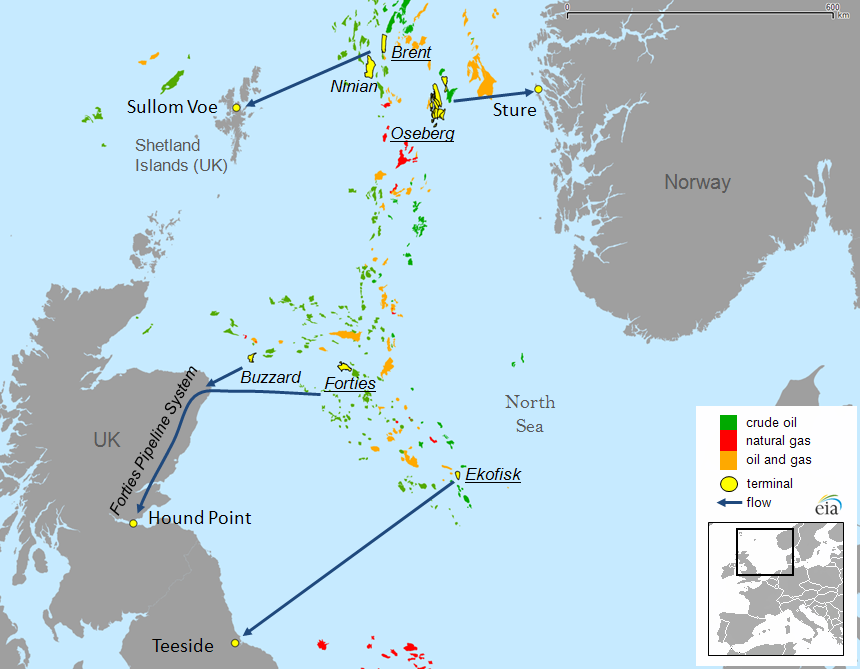
\includegraphics[width=0.75\linewidth]{northseamap}
	%\todo[inline]{Get higher resolution picture}
	\label{fig:northseamap}
	\hbox{\small Source: \thinspace{see footnote\protect\footnotemark}}
\end{figure}
\footnotetext{U.S. Energy Information Administration, United Kingdom Department of Energy and Climate Change, Norwegian Petroleum Directorate}

\subsection{Dynamic Positioning System}
%before making a case for the need of skilled manual manoeuvring operators.
This section describes the dynamic positioning system and its working mechanism. It is background information regarding the scenario that was evaluated. In a gist, dynamic positioning systems automate the task of manoeuvring. But as an automated system, it is not completely fail safe and there have been growing concerns in the industry about over-reliance on DP systems. Hence, it is desirable to have trained human operators capable of manual manoeuvring and, a method for human operators to learn manoeuvring in a superlative manner.

%On-board modern vessels, dynamic positioning system performs the task of manoeuvring automatically. 
%
%Dynamic positioning (DP) is an automated system that helps human operators with manoeuvring operations. 



%With increasing popularity and increased use of sophisticated technology on-board ships, the marine industry can expect more advanced automation in vessel control over the years. Future systems could be enabled with features such as automatic manoeuvring in shallow water and harbour areas, formation sailing, and automatic collision avoidance.

%From early days of the technology where main focus areas of research were accurate position measurement and control system technologies used, research has now moved on to more specialized problems such as optimizing them for energy efficiency.
%The popularity of DP systems has grown to a point where they are a component of medium to large sized vessels these days. 

%This evolution of navigation technology on ships from mere position monitoring systems to automatic position control system has been accompanied by a corresponding growth of specialized personnel responsible for the monitoring of DP systems. 

Position reference systems are vital to the operation of dynamic positioning systems. Information from sensors that provide the vessel’s position and heading along with information from wind sensors, motion sensors and gyrocompasses on the vessel are used to track the vessel and forces acting on it. It is supplied as input to a program that calculates changes in position and heading required to bring the vessel to a pre-set location. The calculation uses a mathematical model of the ship and tries to compensate for unpredictable environmental forces as it decides on power allocations for individual thrusters. While the system takes into account wind forces acting on the vessel measured using wind sensors, a vessel's position is also affected by ocean currents and waves. 
%(refer figure \ref{fig:shipforces})
%Using a mathematical model of the ship and, the forces acting on it, DP system can control the vessel's thrusters to station it in a pre-set location.

% Figure \ref{fig:dparchitecture} is a model of the functional components of a dynamic positioning system. 
%
%\begin{figure}
%	\centering
%	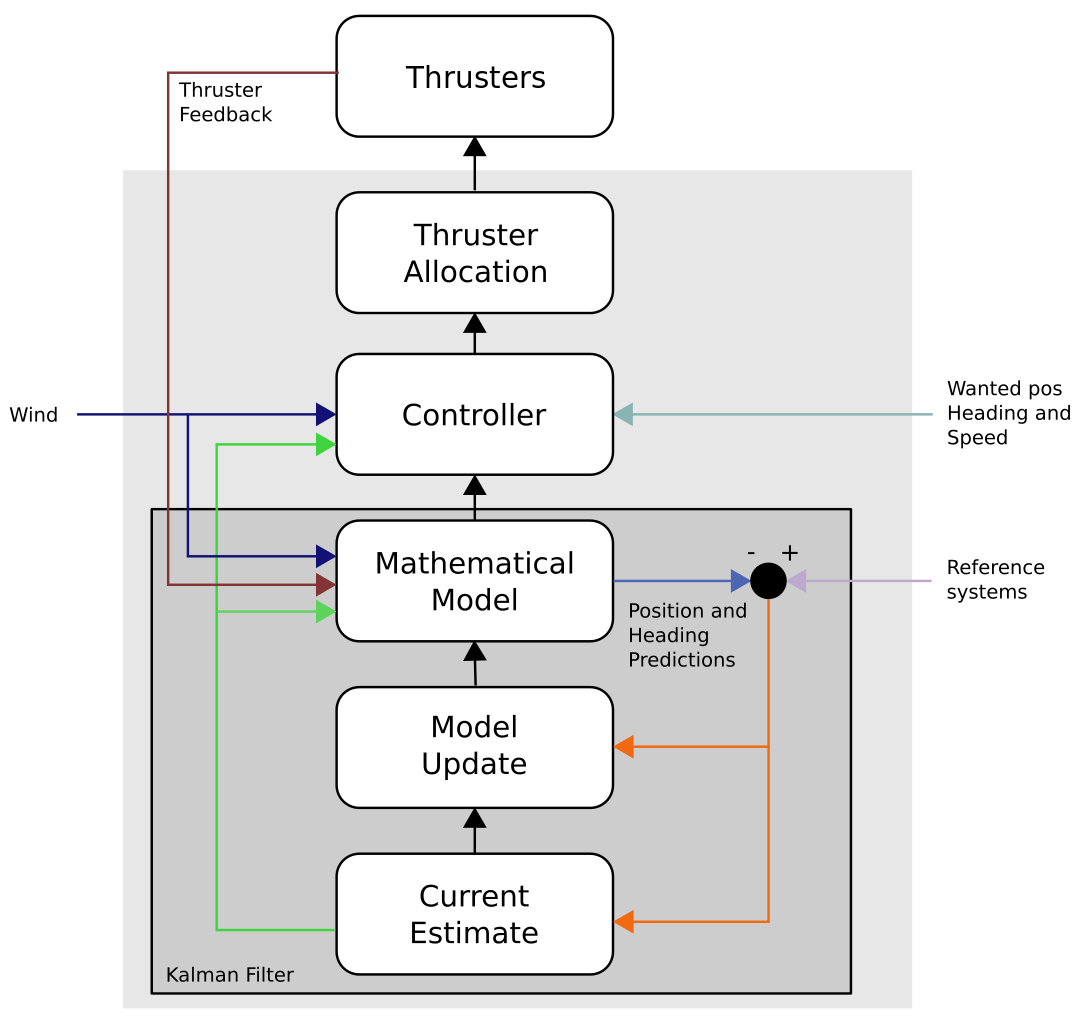
\includegraphics[scale=0.35]{dparchitecture}
%	\caption{Model architecture of Dynamic Positioning systems}
%	\label{fig:dparchitecture}
%\end{figure}
%
%The system contains a \textit{controller} module that influences vessel movements by taking decisions on power allocation for individual vessel thrusters. It takes as input, weather information from wind sensors and current position information from position reference systems. Expected output is to position the vessel at a position and heading preset by the operator. After being initiated, the system determines the difference between current position and desired position. It then attempts to minimize this difference over time. This is done by firing appropriate thrusters into action, producing vessel movements in different directions.  

%\begin{figure}
%	\centering
%	\caption{Forces acting on a ship and its possible movements}
%	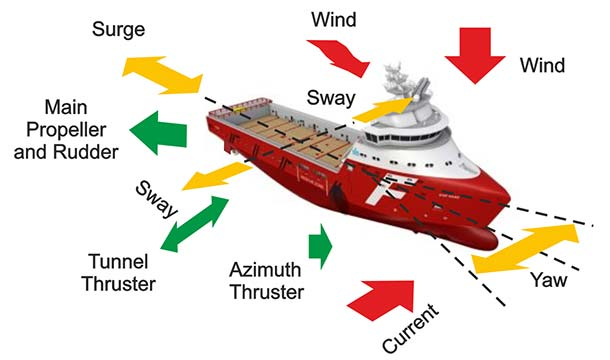
\includegraphics[scale=0.45]{dynamic-positioning}
%	\hbox{\small Source: \thinspace{Kongsberg.com}}
%	\label{fig:shipforces}
%\end{figure}
DP began to be developed as a system that maintains position and heading of a vessel automatically by using its thrusters. DP systems have been increasingly employed over the years and there are well over 2000 DP vessels in operation today \parencite{sorensen2011survey}. Although there do not exist rules specifying acceptance criteria for the positioning performance of DP systems, DNVGL \footnote{Det Norske Veritas (Norway) and Germanischer Lloyd (Germany) - an international certification body} guidelines state that "in moderate weather conditions and with a fully operational DP-system the vessel should generally be able to demonstrate position keeping accuracy with a 3 meter radius and $ \pm $ 1\degree of heading." \parencite{veritas2011dynamic} 

%Kalman filter is generally used to model the environmental forces. It is an algorithm that uses a series of measurements observed over time, containing statistical noise and other inaccuracies, and produces estimates of unknown variables by using Bayesian inference and estimating a joint probability distribution over the variables for each timeframe. While it tends to be more precise than algorithms based on a single measurement alone, it is nevertheless a probability based system that produces estimate predictions of changes in environmental forces over time and some uncertainty in predictions can be expected.

%\todo[inline]{write about accidents that occured. ekofisk etc}

%Figure \ref{fig:praxisdp} shows the interface of a typical DP system. A display monitor is used to show various information regarding the vessel and its control systems. Apart from the display, there exists input interface in the form of buttons. They are used to provide information to the system such as desired location and the mode in which it will be used. 

%\paragraph{Dynamic Positioning Modes}
%
%Most DP systems are offered with several modes of operation. They differ in the type of operation and amount of automation involved. Following are a few common modes of operation. 
%
%%\begin{figure}
%%	\centering
%%	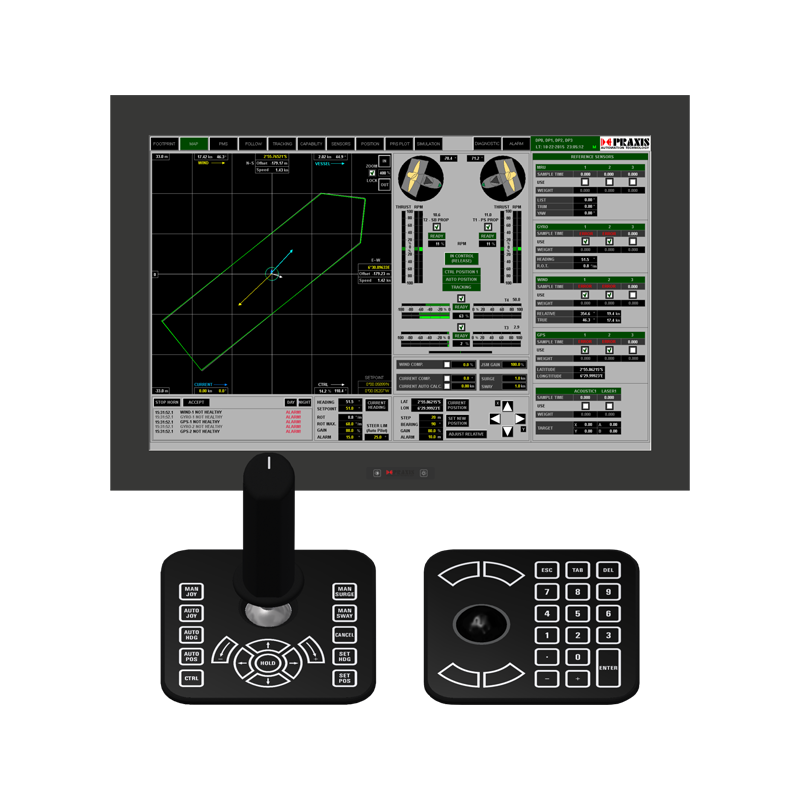
\includegraphics[scale=1]{praxisdp}
%%	\caption{Typical dynamic positioning console}
%%	\label{fig:praxisdp}
%%\end{figure}
%
%\begin{enumerate}[noitemsep]
%
%\item \textbf{Joystick}: Operator can control vessel position and heading manually using a joystick. 
%\item \textbf{Auto heading}: In this mode, the vessel automatically maintains a pre-set heading. 
%\item \textbf{Auto position}: Maintain vessel's position and heading both automatically. 
%\item \textbf{Follow target}: Enables the vessel to follow a moving target. 
%\item \textbf{Autopilot}: In this mode, the vessel steers automatically to follow a predefined course of movement. 
%
%\end{enumerate}
%
%It can be observed that besides functionality, the modes listed above differ by the level of automation involved in the functionality. Joystick mode offers the least amount of automation. In this mode, a single lever can be used to control all of the vessel's thrusters at the same time. A large vessel such as a platform supply vessel typically has two azimuth thrusters at the stern-end of the vessel and one at the bow-end. In addition, they also typically have tunnel bow thrusters that can be used to turn the vessel in place. While it is possible to control each of the thrusters individually from the bridge of the vessel for fine-grained control; the joystick mode encapsulates all the thrusters into one control. This allows control of forward, reverse, steering and even sideways motion using just one lever. 

%\begin{figure}
%	\centering
%	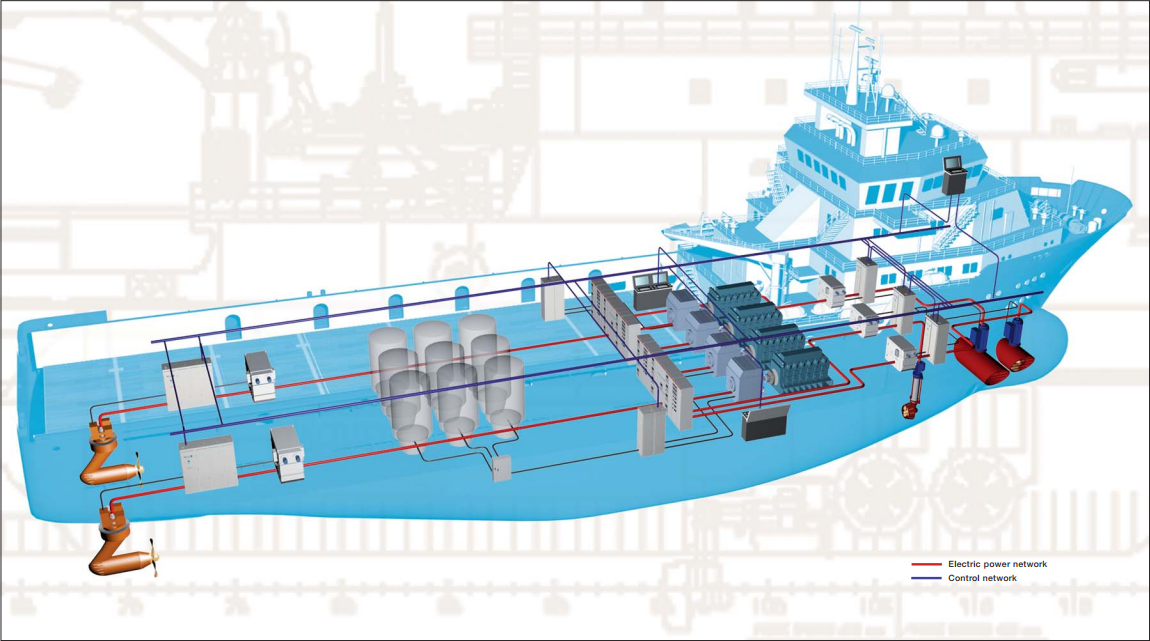
\includegraphics[scale=0.45]{osvlayout}
%	\caption{Schematic diagram of the power and control network of a typical offshore supply vessel}
%	\label{fig:osvlayout}
%\end{figure}

\subsection{Manual Handling}
Going by number of total losses occurring per year (see figure \ref{fig:lossesbyyear}), the safety of vessels world-wide can be said to have improved over the years, particularly in the last decade, despite the ever increasing number of sea-faring vessels. Nevertheless, there is a growing concern in the industry regarding over-reliance on electronic navigation aids. 

\begin{figure}
	\centering
	\caption{Yearly vessel loss since 2005}
	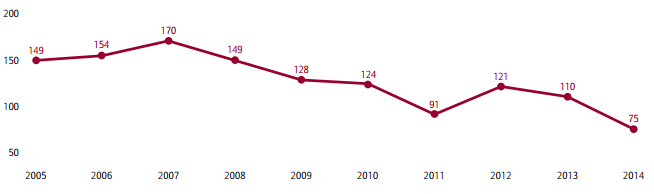
\includegraphics[scale=0.7]{lossesbyyear}
	\hbox{Source: AGCS Safety and Shipping Review 2015}
	\label{fig:lossesbyyear}
\end{figure}

Studies have found human error to be the dominant factor in a significant percentage of the accidents \parencite{baker2005accident, hauff2014analysis}. Incidents such as the Norne shuttle tanker's collision with an FPSO in 2000, standby vessel Far Symphony's impact with the mobile installation West Venture in 2004 and, Big Orange XVIII's collision with the water injection facility Ekofisk 2/4-W in 2009 and  are mentioned as cases of shipping incidents that showcase the lack of preparedness among crew members to handle with emergency situations. \parencite{vinnem2013offshore}.

\section{Operational Demands}
\label{sec:operationaldemands}

Operational demands are an abstraction of the activities that occur in the operation under investigation, which in this case is manoeuvring. Having described the activity itself in the previous section, this section provides an overview of how human operators perform it. The basic skill involved in manoeuvring and the approach taken by maritime professionals to learn it was uncovered by conducting interviews with them. This section describes results of the investigation which in turn drove the specification of a system that can be used to learn ship manoeuvring

A key outcome of the investigation was that an intuitive understanding of vessel handling is required to manually manoeuvre a vessel. Different vessels exhibit different handling behaviour depending on their propulsion technology, steering controls, and, dynamics of the particular vessel owing to its design. These factors have a combined effect on the handling behaviour of the vessel - unique to that vessel-type. Besides, vessels also differ in their response to various weather conditions. 

A clear view of the target object around which the vessel is being manoeuvred provides direct visual feedback of the target’s position relative to the vessel. By looking out the bridge windows, the operator can immediately learn about progress of the manoeuvring operation. Using this information, the operator can make adjustments to the vessel's movement as required. 

Most commercial vessels in excess of size limits determined by local authorities are handled in confined areas by a marine (or maritime) pilot. Marine pilots are seafarers with extensive seafaring experience and are usually qualified master mariners who have been trained as expert ship-handlers. Gaining a high level of intuitive understanding of the vessel’s motion dynamics requires adequate practice. A training system that enables manoeuvring practice on real vessels in real operational conditions is then desirable. It would enable situated learning of ship manoeuvring. 


%\footnote{Refer Appendix for a flowchart of DP certification process (Figure \ref{fig:nidpcertification} )}. One starts with a classroom-based induction course that provides basic knowledge of the principles and practical use of DP. After such a course, the trainee is expected to be familiar with the components of a DP system, concept of redundancy that separate different classes of DP systems, its modes of operation and limitations. Thereafter the trainee goes on to acquire watch-keeping experience on-board real vessels with DP. This watch-keeping exercise takes place for a relatively short period of time where the trainee is familiarised with DP equipments on-board the vessel and gets to witness operations. This is followed by a simulator-based course where the trainee gets practical experience operating DP systems at shore-based simulation centres 


%When manoeuvring large vessels, besides the person at the helm, another person usually aids the operation. Standing outside the bridge of the vessel, this person keeps a lookout for the position of the ship, and conveys it to bridge personnel. He also keeps a lookout for traffic and other objects in the vicinity such as navigational aids.

%\begin{figure}
%	\centering
%	\includegraphics[scale=0.75]{nidpcertification}
%	\caption{Flowchart of nautical institute Dynamic positioning certification scheme}
%	\label{fig:nidpcertification}
%\end{figure} 
%

\subsection{Manoeuvre Training Methods}
Manoeuvre training as it currently happens is reviewed here. It takes place on the job. An inexperienced mariner learns to steer the vessel in navigationally challenging situations by doing it in the presence of a master mariner. The experienced mariner keeps a close eye on the situation as the apprentice learns by doing. During the course of operation, the apprentice receives guidance and feedback on performance. 

This type of learning can be classified as experiential learning. According to this theory, learning is a "continuous process grounded in experience" \parencite{kolb2005learning}. When it comes to ship manoeuvring, learning it on the job must have sufficed in past times. However, developments in offshore energy exploration have place a greater emphasis on ship manoeuvring. 

A drawback of on-the-job training is that it does not allow for repeated practice in a controlled environment. Also, the learning is not systematic in that it takes place on a need basis with no objective grading of learning outcomes. Simulator-based training may also be used to learn manoeuvring, but ship motion behaviour in simulations is artificial and the learning is not grounded in reality. Augmented reality-based on-board training can provide for training environments where manoeuvring can be learnt methodically. A learning framework may be introduced where specific manoeuvring skills are identified along with best practices for executing them. In such a framework a trainee may build competence incrementally. Table \ref{tab:comparetrainingmethods} presents a comparison of simulator-based training, mixed reality on-board training and practice-based or on-the-job learning. 

\renewcommand{\arraystretch}{1.2}% Wider
\begin{table}[linewidth]
	\centering
	\begin{tabular}{p{4.5cm}|P{2.0cm}|P{2.2cm}|P{2.0cm}@{}}
		\toprule
		\multicolumn{1}{c|}{ } & \multicolumn{1}{P{2cm}|}{\textbf{Simulator}} & \multicolumn{1}{P{2.2cm}|}{\textbf{AR on-board}} & \multicolumn{1}{P{2cm}}{\textbf{On-the-job}} \\ 
		\midrule
		Practice on actual vessel in real conditions                         & \xmark                            & \cmark                                        & \cmark                                        \\
		Practice in various weather conditions     & \xmark                            & \cmark                                        & \cmark                                        \\
		Perform training repetitions in same conditions & \cmark                            & \xmark                                        & \xmark                                        \\
		Scope for standardized competency assessment    & \cmark                            & \cmark                                        & \xmark                                        \\
		Scope for gradation of learning outcomes   		& \cmark                            & \cmark                                        & \xmark                                        \\
		Close range ship handling training              & \cmark                            & \cmark                                        & \xmark                                        \\
		Scope for introduction of learning framework    & \cmark                            & \cmark                                        & \xmark                                        \\
		Risk of collision with other vessels            & \xmark                            & \cmark                                   		& \cmark                                        \\
		Suitable for learning level                     & All                               & All		                               & Advanced       \\
		\bottomrule                         
	\end{tabular}
	\caption{Comparison of training methods}
	\label{tab:comparetrainingmethods}
\end{table}

\subsubsection{Ship Simulators}
Among other uses, maritime industry found use for computers as devices that could be used for the simulation of movements of vessels on sea. In a gaming-like use case, computers are used to run ship simulation software for educational purposes. These programs can be used to control virtual ships in virtual marine environments. Some set-ups involve actual bridge equipment to input commands to the program, making the experience more realistic. An array of monitors are used for display. Backed by computer graphics and models of sea, vessel and other objects, the simulation software is supposed to create the perception of being inside a real vessel. It is now standard practice to undergo training using simulators in the maritime industry. Figure \ref{fig:vstepdpsim} shows the set-up of a typical dynamic positioning simulator. 

\begin{figure}
	\centering
	\caption{Dynamic positioning simulator}
	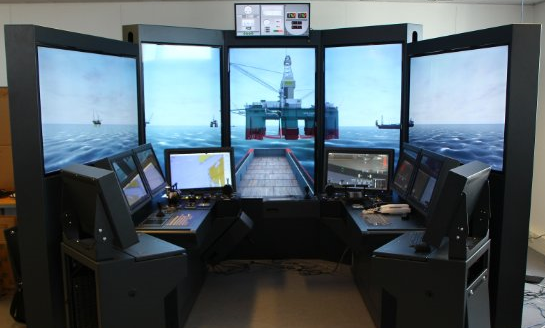
\includegraphics[width=0.7\linewidth]{vstepdpsim2}
	\hbox{\small Source: vstepsimulation.com}
	\label{fig:vstepdpsim}
\end{figure}


\section{Human Factors Knowledge}
\label{sec:humanfactors}
\subsection{Mode Errors}
Mode errors are the errors that occur when a user operates an interface in a manner that is appropriate to a different state of the system than the one it actually is in. When the user forgets the actual state and performs an action appropriate to a different state, the system response is unexpected and usually undesired. A common example of mode errors is the undesired input of capitalised letters on a computer due to caps lock, or the inability to enter numbers using the number pad due to numlock. 

The design of a ship operation training method set in augmented reality needs to take into account the possibility of mode errors resulting from the two realities that are simultaneously at play. A trainee moving a real ship in augmented reality is also moving it in actual reality. Take the example of a training exercise to approach a virtual object out in the open sea. In the course of the exercise, the trainee moves the vessel towards the virtual object in the augmented reality. At the same time, the real vessel is actually moving somewhere out in the open sea. If the bridge equipment is also augmented, the radar would be expected to display an indication of the virtual oil platform. Adding a virtual object to a radar display that already contains information regarding other real objects can be confounding to users (figure \ref{fig:nocolour}). A way to distinctly identify virtual objects (for example, figure \ref{fig:diffcolour}) should help reduce mode errors but it also hampers immersion of the experience. 

\begin{figure}
    \centering
    \begin{subfigure}[b]{0.45\textwidth}
        \centering
        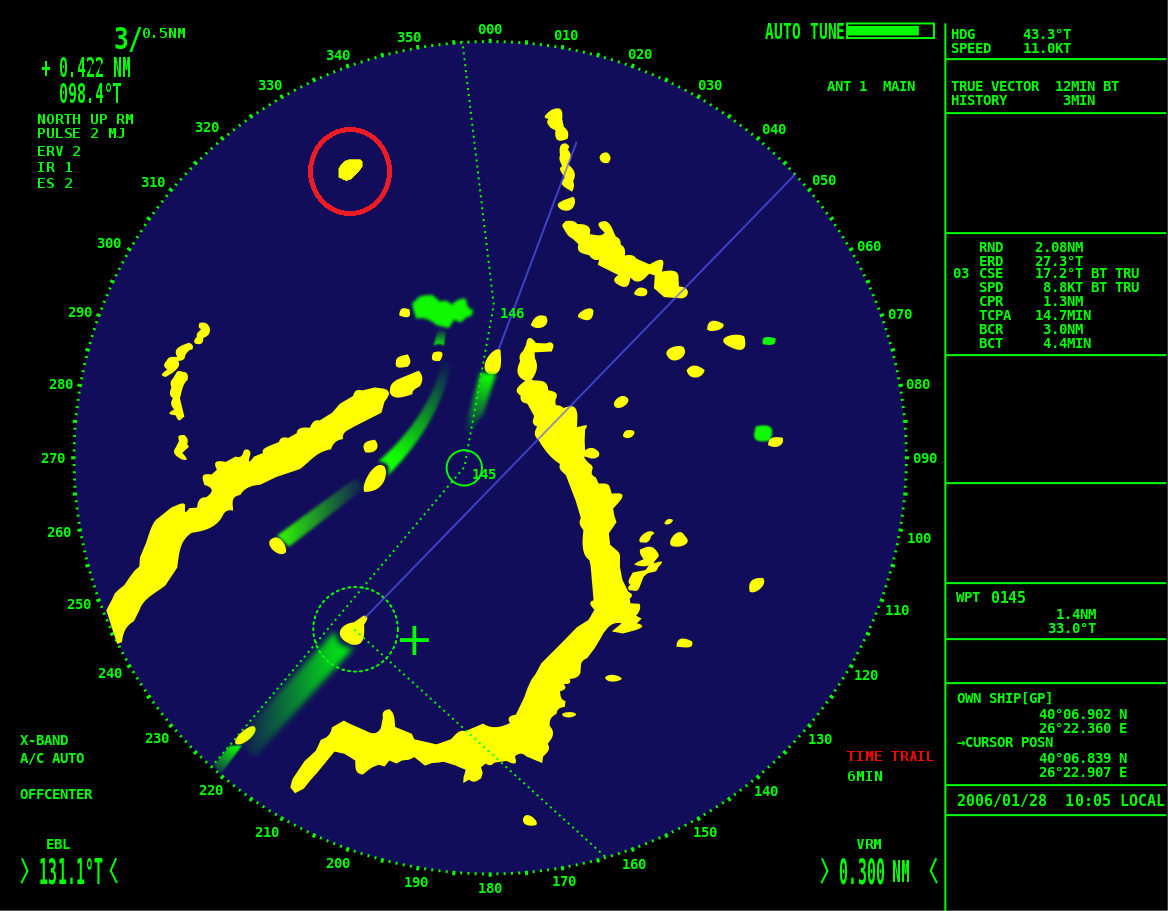
\includegraphics[width=\textwidth]{radarOrig1}
        \caption{No colour differentiation}
        \label{fig:nocolour}
    \end{subfigure}
    \hfill
    \begin{subfigure}[b]{0.45\textwidth}
        \centering
        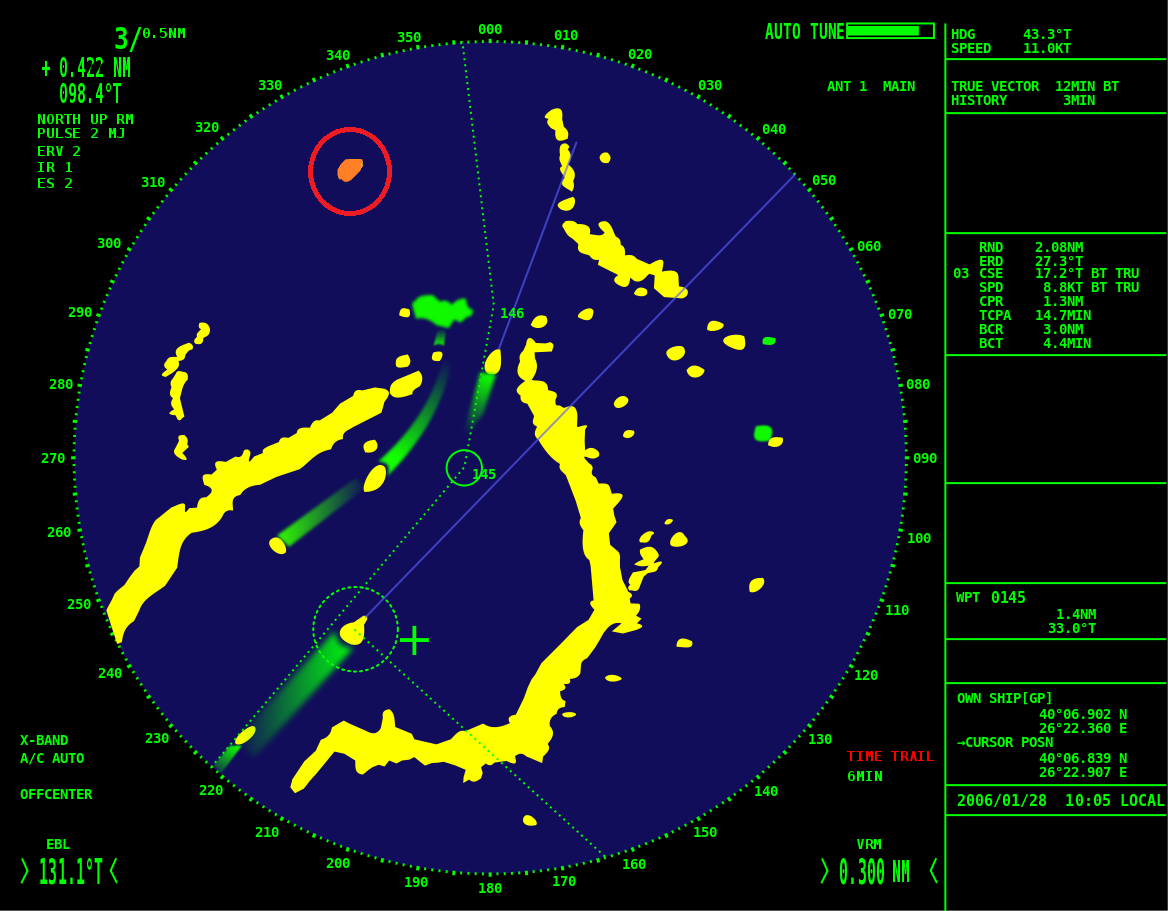
\includegraphics[width=\textwidth]{radarOrig2}
        \caption{Differentiated virtual object}
        \label{fig:diffcolour}
    \end{subfigure}
    \caption{Display of virtual objects on radar}
    \label{fig:threegraphs}
\end{figure}

\section{Envisioned Technology}
\label{sec:envisionedtech}
An important choice in the design of a new human-computer interface is the technology used to build prototypes, and eventually the end product. This section describes two technical choices made for the implementation of a prototype. They fulfil display and tracking requirements that are part of an augmented reality system. Choices were made based on investigation of literature on the subject and surveying the state-of-the-art consumer devices commercially available at the time of the research.

%For example, devices like keyboard, mouse and trackpad have acted as the standard input interface for personal computers for over 2 decades now, while computer monitors in the form of CRT, LCD and TFT displays have formed the output interface. Not unlike television monitors, computer monitors were initially used for purposes of data processing before being used for entertainment purposes such as gaming and media streaming. The evolution of computing technology from large machines driven by punch cards and that filled up entire large rooms to the personal computer form goes hand in hand with their ubiquitous use in the modern world influencing the manner in which most office jobs are carried out today. 
%
%Computers had a significant impact on the maritime industry. Where naval architecture was traditionally a craft with little scientific information to back designs, modern computers enabled computing power to be leveraged to predict performance. Modern ship designs make use of tools that have been developed to assess static and dynamic stability, water resistance, for hull development and structural analysis. 

\subsection{Augmented Reality Display}
This section is about display technology needed to create augmented reality applications. It describes different options for creating the visual perception that is part of augmented reality. Further, the utility of the displays for ship handling training is argued. 

Three types of augmented reality displays were first catalogued by \cite{azuma1997survey} - namely, optical see-through, video see-through head-mounted displays and, spatial augmented reality. Optical see-through displays allow an unhindered view of the outside world in theory, whereas in video see-through display the user's view is camera-mediated. In comparison, optical see-through HMD appears to be the logical choice for AR and was chosen for prototyping. It is ideologically consistent with AR in that most of the visual reality is left untouched only to add bits of information (real/virtual) as necessary. A more detailed comparison of the utility of optical and video see-through display is presented in section \ref{sec:ostvsvst}. Spatial augmented reality is another option for AR, but the lack of mobility makes it infeasible in this scenario. It is nevertheless described in brief here for posterity. The following sections briefly describes each before comparing optical and video see-through HMDs. For an in-depth coverage of the concepts, readers are referred to \cite{azuma1997survey}, \cite{azuma2001recent} and \cite{zhou2008trends}.

\subsubsection{See-through Display}
In general, see-through displays allow the user to see the real world through a display system while also being able to seamlessly display digital content on it. These were first developed for military aircraft for applications such as fixing the target of ammunition on locations that could be seen through the aircraft. Such display systems can also be mobile with users wearing them on the head so as to directly influence their view of the outside world. These are called as head-mounted displays (HMDs). The following sections describe optical and video see-through displays in turn. A comparison of the two technologies presented thereafter.

% The concept of see-through display is also making way into consumer markets with head-up displays used in cars being a more popular use. 

\paragraph{Optical See-Through HMD}
Optical see-through head-mounted displays (OST) are display systems that exploit the transparency of glass material to provide unobstructed views of the outside world. By definition, they can also digital content on the same surface simultaneously. OST displays use optical combiners to combine light from the real world with digital content. Optical combiners usually reduce the amount of light from the real world. Combiners act like half-silvered mirrors to be able to reflect light from monitors into user's eyes. Theoretically, this display system can provide an undistorted view of the real world (apart from slight obstructions caused by the glasses' frame itself). As a downside, it also affects the display of digital content adversely, making virtual objects appear semi-transparent and 'ghostlike'.

%\begin{figure}
%	\centering
%	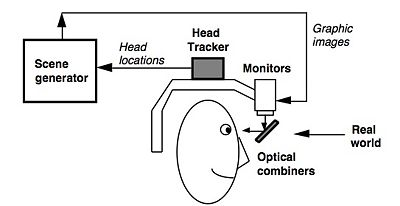
\includegraphics[width=\linewidth]{opticalseethrough}
%	\caption{Schematic diagram of optical see through display (Source: \cite{azuma1997survey})}
%	\label{fig:opticalseethrough}
%\end{figure}

\paragraph{Video See-Through HMD}
Video see-through HMDs are similar to optical see-through HMDs in that they allow the combining of real world views with digital content. Differences between them stem from their source of real world view. As opposed to OST which provides a direct view of the environment, VST uses video feed from a camera in the HMD system to provide real world views. So, in addition to the head trackers and viewing monitors as in OST, VST HMDs require a camera appendage in the setup. The video camera mounted on the exterior of such an HMD incorporates external view back into the content. This type of HMDs obscures the wearer's external view in favor of better immersion into the stereoscopic view provided by the system. 

\subsubsection{Optical vs Video See-Through Display}
\label{sec:ostvsvst}
This section provides a comparison of optical and video see-through HMDs based on parameters thought to be relevant to this study. For an in-depth review and comparison between these two display types, readers can refer to \cite{rolland1995comparison}. Table \ref{tab:comparehmds} (see appendix) presents a comparison of the see-through displays on various parameters.


\paragraph{Simplicity} 
In addition to virtual images, there is a need to view the external world in augmented reality applications. Optical see-through systems meet this requirement naturally by employing transparent displays which do not interfere with the outside view. Video see-through systems on the other hand, obscure the outside view and need to use a camera that is looking outwards to compensate. The camera then seeks to perform the role of human vision - one of the most complicated sensory systems in the universe, the various functions of which are either not built into or not yet achievable using consumer grade cameras. For example, the resolution of the entire view (real + virtual) is limited to that of the display device in case of VST. This constraint is also present in optical see-through devices, with a crucial difference that it is only applicable to virtual parts of the scene. 
	
\paragraph{Lag}
A persistent problem with interactive computer graphics is that of time delay (lag) between expectation of the appearance of a scene and it's actual appearance. In an OST system, there will be near zero lag in viewing real scene as it is viewed directly by the user. Whereas, the display of any virtual objects can be a source of lag. The system first needs to decide whether to display virtual objects based on viewing direction and orientation and, also calculate appropriate projection of the virtual object if and when it is to be displayed indeed. Finally, there will be a small delay in rendering images on the display system. 

In VST, additional lag is present in digitizing video stream of the real world. In a display that refreshes at 60Hz, the time that elapses between display of one frame and another is 16.67ms. Hence there will be a minimum of 16.67ms delay in displaying the external view recorded by a camera, discounting the time taken to digitize the camera view. According to \parencite{ellis1997factors}, for close range tasks, one millisecond of delay causes one millimeter of error. One advantage of VST over OST is that the higher degree of control over display streams (real and virtual) in video see-through makes it possible to avoid the problem of temporal mismatch due to delay in virtual images by delaying real view as well. But then delaying display of real-world view affects proprioception which is intolerable in this scenario as manoeuvring requires timely, fine adjustment of ship controllers.
	


%Low-cost HMDs are available in the consumer market and can be used for 3D games and entertainment applications. With the addition of one or two cameras, these can be leveraged for mixed reality applications. 

%Consequently, calibration of the camera's view to that of the user's eye position will have to be made.

%Driven by interest from the gaming community, and virtual reality applications in general, closed-view HMDs have seen more development as of this writing compared to optical see-through displays. 
%\begin{figure}
%	\centering
%	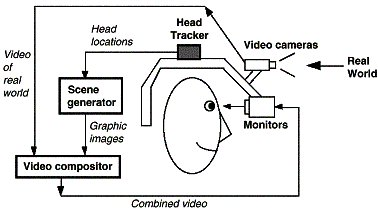
\includegraphics[width=\linewidth]{videoseethrough}
%	\caption{Schematic diagram of video see through display (Source: \cite{azuma1997survey})}
%	\label{fig:videoseethrough}
%\end{figure}

\subsubsection{Spatial Augmented Reality}

Spatial augmented reality (SAR) refers to the concept of augmenting real-world spaces (with digital media) without the use of special devices such head-mounted display \parencite{bimber2005spatial}. A discussion of display options for AR would be incomplete without spatial augmented reality. However, the lack of standardized solutions and the need to set up special hardware tailored to individual ships makes SAR an impractical solution for the creation of AR on-board ships for manoeuvring training purposes. Nevertheless, the concept is described in brief here for completeness. A detailed treatment of the topic of spatial augmented reality can be found in \cite{bimber2005spatial}.

\paragraph{Conceptual Overview}
Alongside HMDs, spatial augmented reality forms another paradigm for the creation of mixed reality content. In SAR, the user experiences augmented reality through one or more monitors placed in front, displaying a combination of virtual and real-world images captured by video camera. This is similar to the CAVE \parencite{cruz1993surround} concept for virtual reality. CAVE (CAVE automatic virtual environment) seeks to immerse the user in a 3D virtual environment created using rear/front facing projectors lighting up projection screens in three dimensions. Although originally designed for virtual reality experience, the concept can be adapted for augmented reality. Advances in projection technology make it possible to have projections on transparent screens \parencite{peterson2006human}. 

\paragraph{Advantages}
SAR offers unique benefits over HMDs such as obviating the need for users to wear special devices and possibly high resolution, wide field of view displays integrated into natural environments. Large field of view and higher resolution provides a stronger feeling of presence \parencite{lantz1996future}, allowing for better immersion and easier eye accommodation\footnote{refer to section \ref{sec:photorealism} for a discussion on photorealism}. 

\paragraph{Disadvantages}
On the downside, it suffers from setbacks such as requiring setting up of expensive custom-made display configurations that need more space and hardware than standardized HMDs. A portable technological solution that enables mobility between vessels is desired. This allows for training to be conducted on various different vessels with minimal time and effort involved in setting up the augmented environment. Using mobile AR devices such as HMDs enables trainees to bring their own AR devices on-board and vessels do not need to be docked for purposes of setting up the AR environment.

%Figure \ref{fig:monitorseethrough} shows a concept of monitor-based spatial augmented reality. 



%\begin{figure}
%	\centering
%	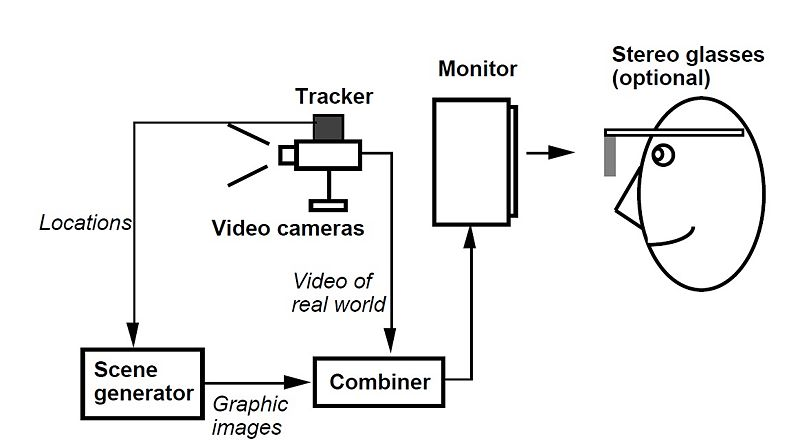
\includegraphics[width=\linewidth]{monitorseethrough}
%	\caption{Schematic diagram of monitor see through display (Source: \cite{azuma1997survey})}
%	\label{fig:monitorseethrough}
%\end{figure}

\paragraph{In Conclusion}
As opposed to head-mounted displays, SAR relies on projectors to create the views necessary for the perception of mixed reality. SAR may be just as effective as head-mounted displays in being able to create immersive mixed environments. A study on the use of large projection screen as an alternative to HMDs for virtual environment found no significant difference between the two for spatial cognition tasks \parencite{patrick2000using}. But projector-based display systems are custom solutions that need to be designed for the specific environment in consideration. Ships come in a variety of shapes and sizes, so do their bridge rooms. Setting up AR environments on-board new vessels will need considerable effort to tailor the display system for individual ship. Besides, some modification of the ship's bridge room is involved such as placing of projectors at appropriate locations and turning bridge windows into projection screens onto which virtual objects can be projected. The operation down-time needed to create custom display solutions for individual ships is expensive and undesirable.


%The display technologies considered so far have been applicable for creation of mixed reality for individual users. These systems do not scale easily to groups of users needing to experience the same mixed reality. For example, in the mixed reality ship handling training method that is being conceived in this project, it is required that at least two people experience the same scenario, i.e. the trainee and a trainer (experienced ship handler). Apart from the trainee who needs to view the virtual object/s for training purposes, the trainer also needs to see the same in order to evaluate trainee performance. Collaborative design such as for architecture and modeling is another use case multiple users needing to experience the same mixed reality. 
\subsubsection{A Note on Photorealism}
\label{sec:photorealism}
Photorealism in this context refers to the quality of visualisation of objects in the simulation. At high levels of photorealism, virtual objects are visible with a high level of detail, blend seamlessly into the surroundings - appropriately occluding objects behind it and, are of proper focus and contrast, with the end result being a realistic visualisation whose virtual aspects are hard to distinguish from the real. 

%Stereoscopic displays are plagued by problems from accomodation-vergence conflict \parencite{hoffman2008vergence}. 

For purposes of this study, photorealism is grouped into three distinct levels. One of the attributes on which the classification has been made is the extent to which accommodation-vergence conflict affects a scenario. Another attribute is occlusion, an essential depth cue that can be important in manoeuvring scenarios for instance. Table \ref{tab:trainingoptions} is a listing of the three categories.

\subsection{Ship Instrument Augmentation}

Augmented reality displays described in the previous section form a part of the enabling technologies for the mixed reality ship manoeuvring training envisioned in this research. HMDs for instance can help create visual perception of an offshore oil platform standing on the open sea. In other training scenarios they may be used to display tracks/lanes for navigational tracking or virtual ships on collision course/sailing side-by-side etc. Different artefacts may be displayed depending on training objectives and the perceptions that need to be created. Ships over the years though have evolved to be technically complex machines. The bridge room of a modern age vessel houses multiple instruments tracking different aspects of its reality. Therefore, the design of a mixed reality environment on-board a modern seafaring vessel should consider how virtual objects interact with various instruments in the bridge room to accurately correspond with the reality that is being visually perceived.  
%
%\subsubsection{Bridge Instrumentation}
%

\subsection{The Tracking Requirement}
Tracking is a vital requirement for augmented reality, needed to fulfil the requirement that virtual objects be registered in three dimensions. This section describes the tracking requirement and a design choice made in that regard. Two types of tracking solutions are described along with their implications for the on-board training scenario. For a detailed discussion of tracking methods, readers are referred to \cite{zhou2008trends}. According to \cite{zhou2008trends}, tracking, being a core enabling technology for AR, is an unsolved problem with many "fertile" areas of research.

An AR system needs vision capability in order to track viewer’s position and register objects in his field of view. Specifically, it is of interest to track user's head position and gaze direction so that virtual objects can be placed in the appropriate location. Tracking systems usually comprise of camera/s that are used to sense real-world space. Cameras produce the raw data necessary for computer vision systems.   

Tracking solutions can be one of two categories - outside-in and inside-out tracking, or a hybrid solution of them.  The two types differ based on the positioning of camera relative to viewer. Inside-out tracking systems are those in which camera is placed on the viewer and it tracks the environment as he/she moves around in it. Whereas in outside-in tracking, a stationary camera that is placed away from the viewer (but in sight and, without occlusion) tracks the viewer’s movement using markers placed on the viewer themselves. Outside-in tracking was chosen as the method of tracking in this study as it needs significantly lesser modification of the environment in which the tracking takes place compared to inside-out tracking. Moreover, outside-in tracking is considered to be more accurate at tracking position than inside-out tracking systems \parencite{klein2006visual}. 
%It is common for tracking systems to work on the infra-red light spectrum even though the concept is also viable on the visible spectrum.

\subsubsection{Inside-out Tracking}
Inside-out tracking refers to systems in which the camera that tracks positions is located in the same physical location as the device/viewer being tracked (head mounted display for example) so the camera moves along with the tracked object. With the camera mounted on the object that is being tracked, the system tracks the world around it from the vantage point of the tracked object. Changes in location/orientation of the tracked object can be detected from the camera’s changing perspective of the outside world.

A straightforward implementation of this idea would process images from video stream captured by the camera to locate objects in the world space and register virtual objects among them. However, interpreting live camera feed is a computationally expensive operation due to the difficult computations involved in processing images on the fly. 

\paragraph{Fiducial Markers}
A popular refinement of this technique is to place so called fiducial markers in the environment being tracked. Figure \ref{fig:eiffel_marker} shows a typical marker that can be used for marker-based tracking. Visible markers (to camera) in the tracked space reduce the complexity of image processing computations. The tracking system is then aware of the type of images to look for and make decisions accordingly. Moreover, marker images are usually black-and-white in order to simplify image processing computations by converting raw camera output to black-and-white. 

\begin{figure}[linewidth]
	\centering
	
\includegraphics[scale=0.5]{eiffel_marker}
	\caption{A typical fiducial marker}
	\label{fig:eiffel_marker}
\end{figure}

\subsubsection{Outside-in Tracking}
Outside-in tracking systems are those in which a stationary camera placed away from the viewer in the tracking environment tracks the viewer. Changes in viewers position are tracked using markers placed on them. Unlike inside-out tracking systems, tracking range with this method of tracking is not limited by fiducial markers in the environment. 

A disadvantage with this system is that since the camera is at a different physical location than the system that generates the virtual images, tracking data is not directly available on the AR system itself. Then data has to be sent to the system from a separate device that does the tracking. Data can be sent by a wireless or wired connection. A wired connection impedes free movement in the environment but it is also the faster and more reliable method of data transfer. Data might also be sent wireless which allows for ease of movement. But it comes at the cost of latency and reliability issues in data transfer. 

Besides latency in obtaining tracking information on the AR headset, another disadvantage of this tracking system is that it is susceptible to noise in the form of ambient infra-red light. This is a constraint on the system with the implication that lighting in the tracked space will have to be carefully controlled to prevent the system from being affected by noise.

\paragraph{In Conclusion}
Outside-in tracking was chosen as the method of tracking for this scenario. This method of tracking allows for the creation of a tracking system with minimal changes to the environment in which the tracking takes place as there is no need to place fiducial markers. It is required to have a clear view from the bridge of the vessel for safety reasons. Markers obscure external view since they will have to be placed on the window of the bridge in order register a virtual object in that region of space.
